\thispagestyle{toanhocvadoisongnone}
\pagestyle{toanhocvadoisong}
\everymath{\color{toanhocdoisong}}
\graphicspath{{../toanhocdoisong/ori/}}
\begingroup
\blfootnote{$^1$\color{toanhocdoisong}Viện Sinh học và Môi trường Đông Dương.}
\AddToShipoutPicture*{\put(0,616){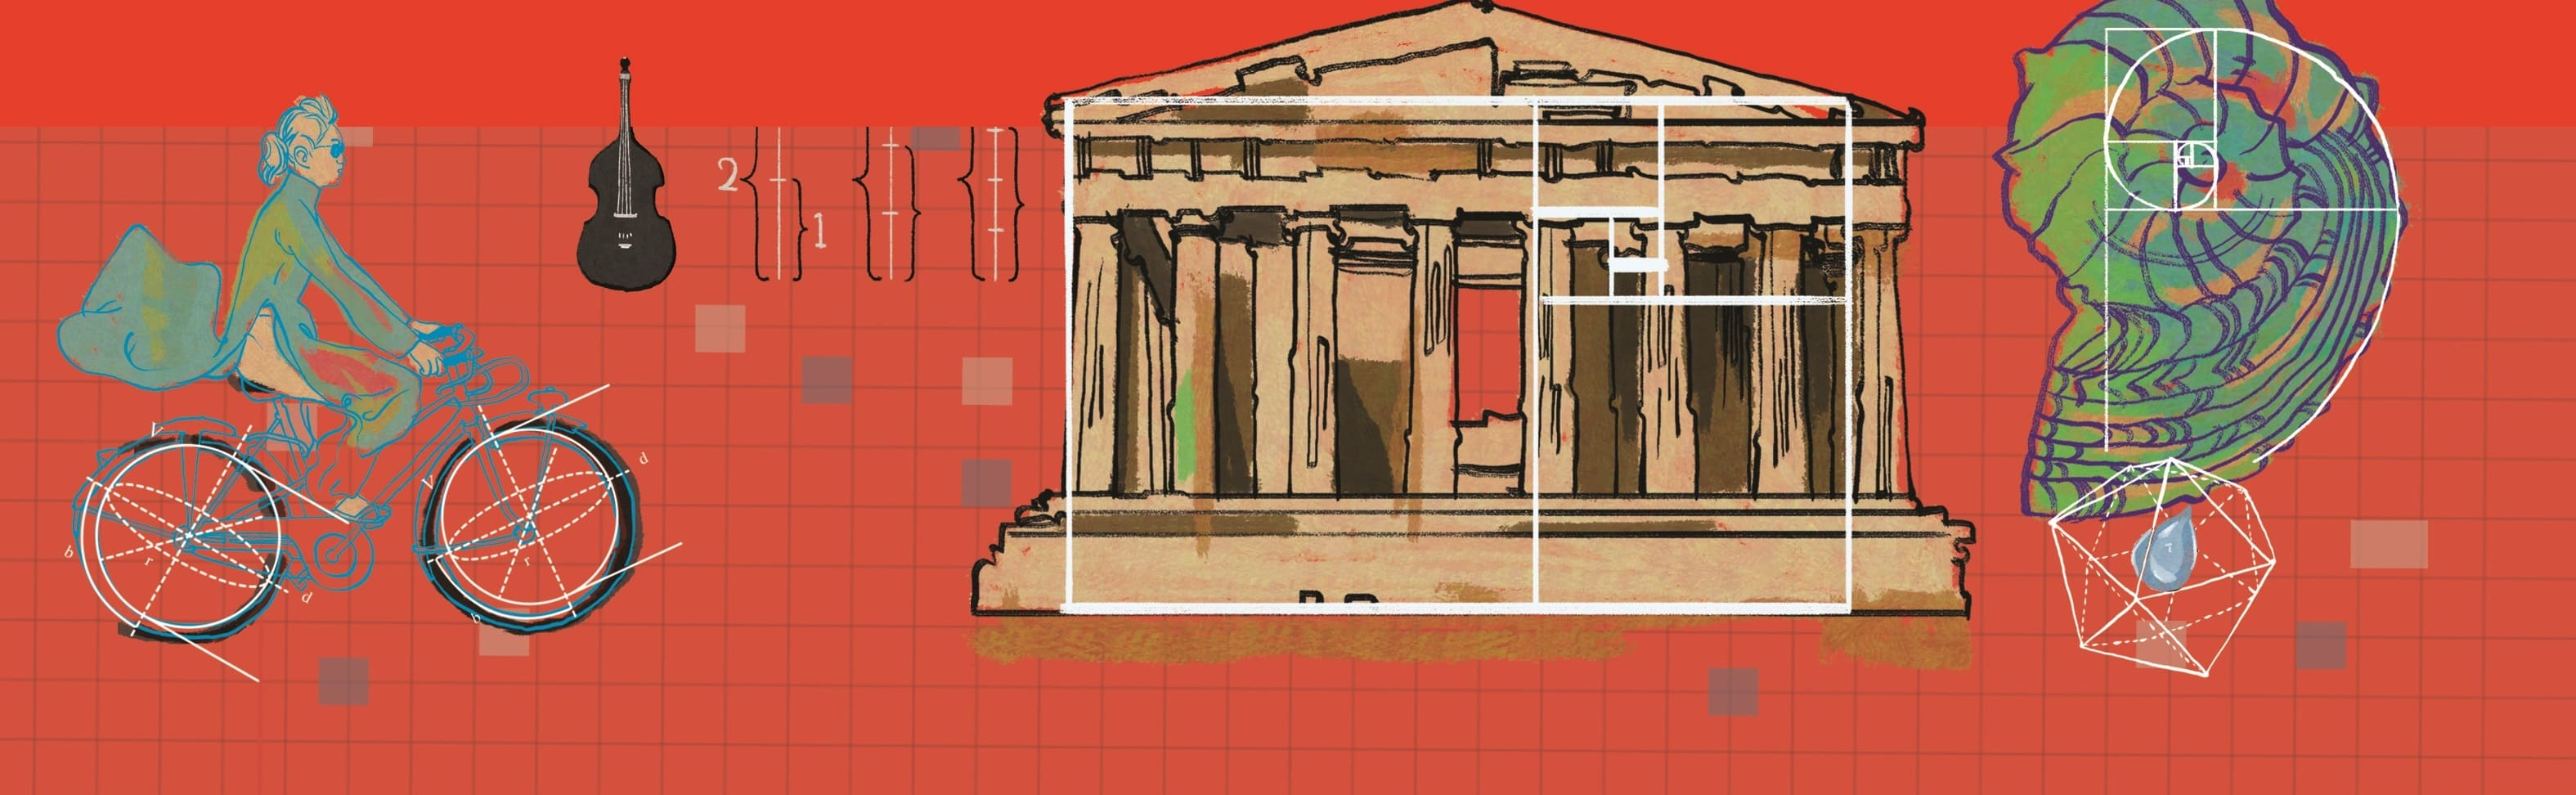
\includegraphics[width=19.3cm]{../bannertoanhocdoisong}}}
\AddToShipoutPicture*{\put(88,520){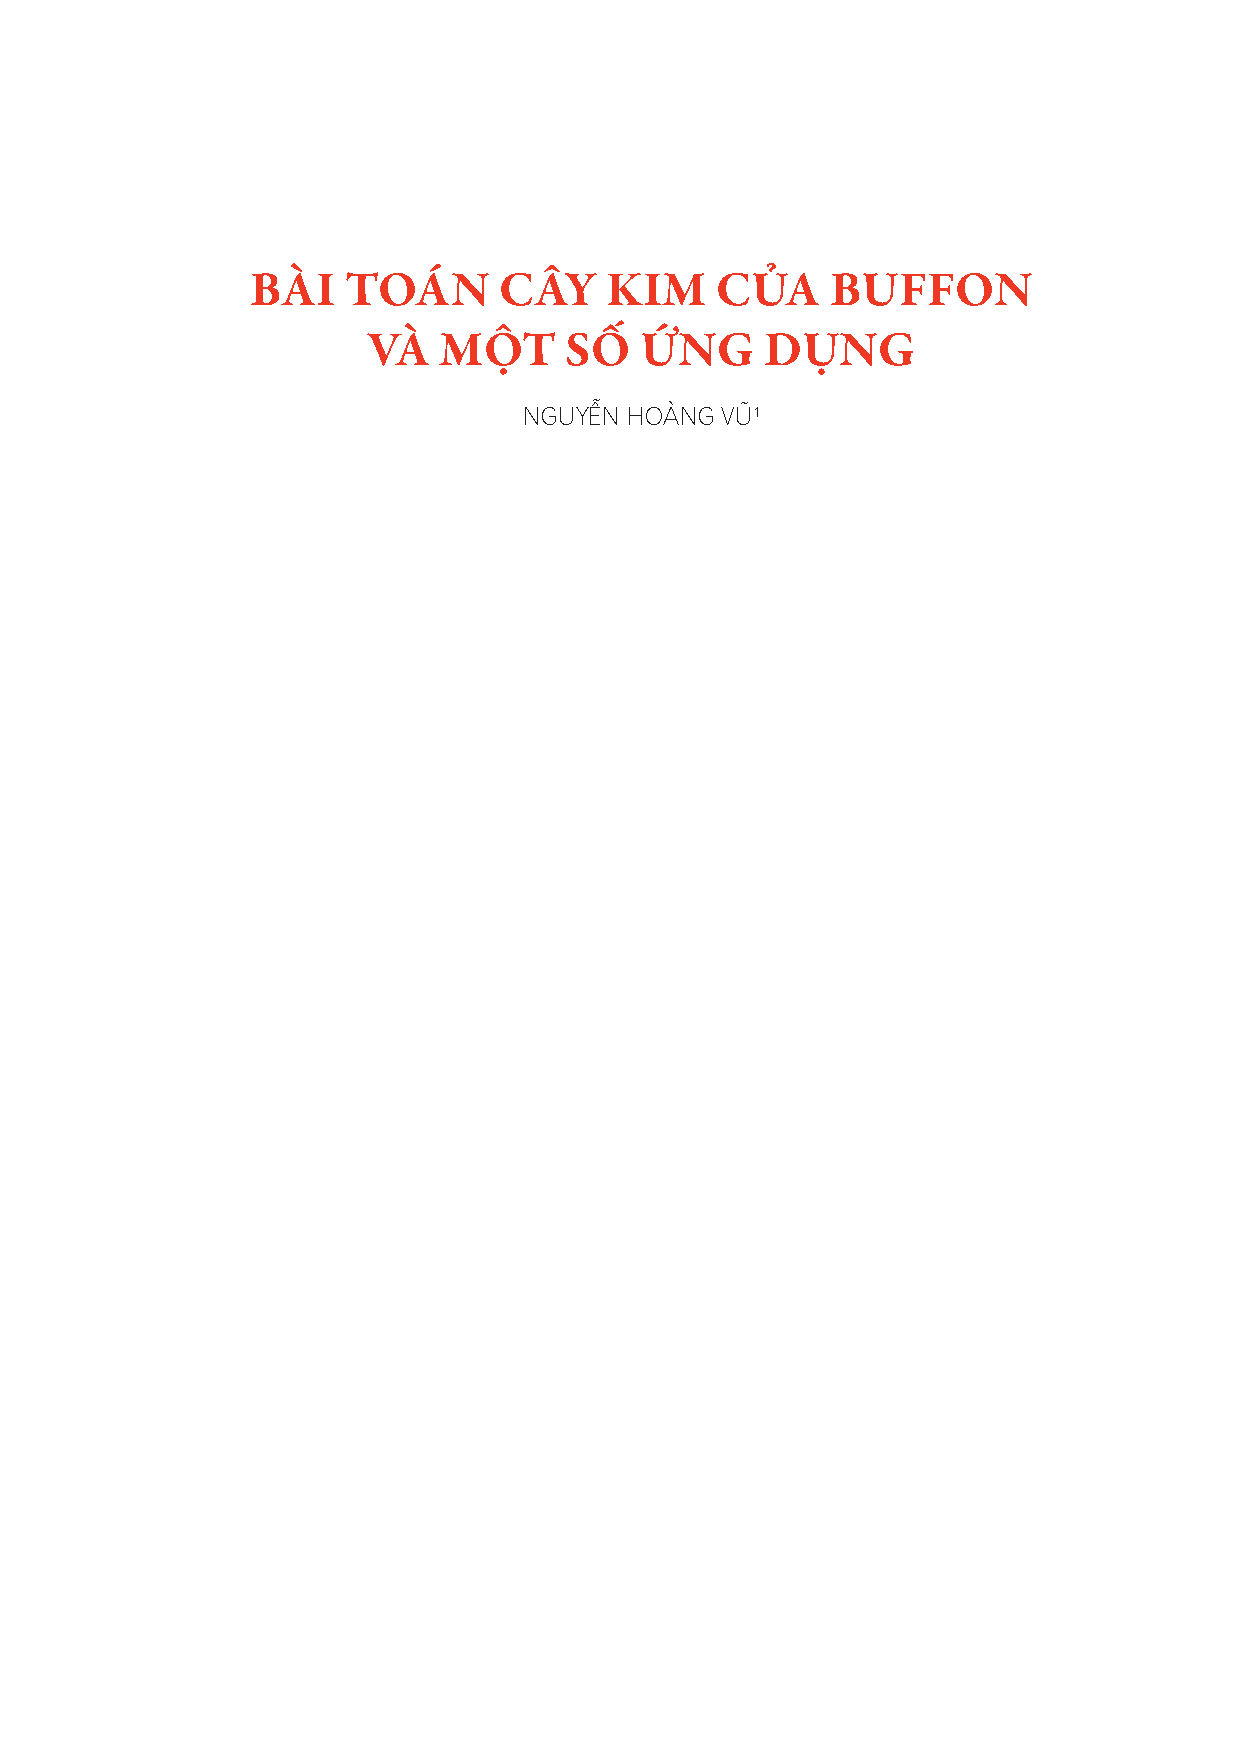
\includegraphics[scale=1]{../tieude.pdf}}}
\centering
\endgroup

\vspace*{190pt}

\begin{multicols}{2}
	\setlength{\abovedisplayskip}{4pt}
	\setlength{\belowdisplayskip}{4pt}
	$\pmb{1.}$ \textbf{\color{toanhocdoisong}Quan hệ giữa các góc của nếp gấp}
	\vskip 0.1cm	
	Với mỗi nếp gấp trong origami, ta xét đến hai mặt phẳng chứa các phần tờ giấy kề với nó. Hai mặt phẳng này sẽ nhận nếp gấp làm giao tuyến. Người ta quy ước góc ứng với mỗi nếp gấp là khoảng cách góc của hai mặt phẳng này so với trạng thái được trải phẳng. Tức là, góc này nhận giá trị $0^\circ$ khi hai mặt phẳng đồng phẳng, $180^\circ$ khi nếp gấp được gập lõm hoàn toàn và $-180^\circ$ khi nếp gấp được gập lồi hoàn toàn.
		\begin{figure}[H]
		\vspace*{-5pt}
		\centering
		\captionsetup{labelformat= empty, justification=centering}
		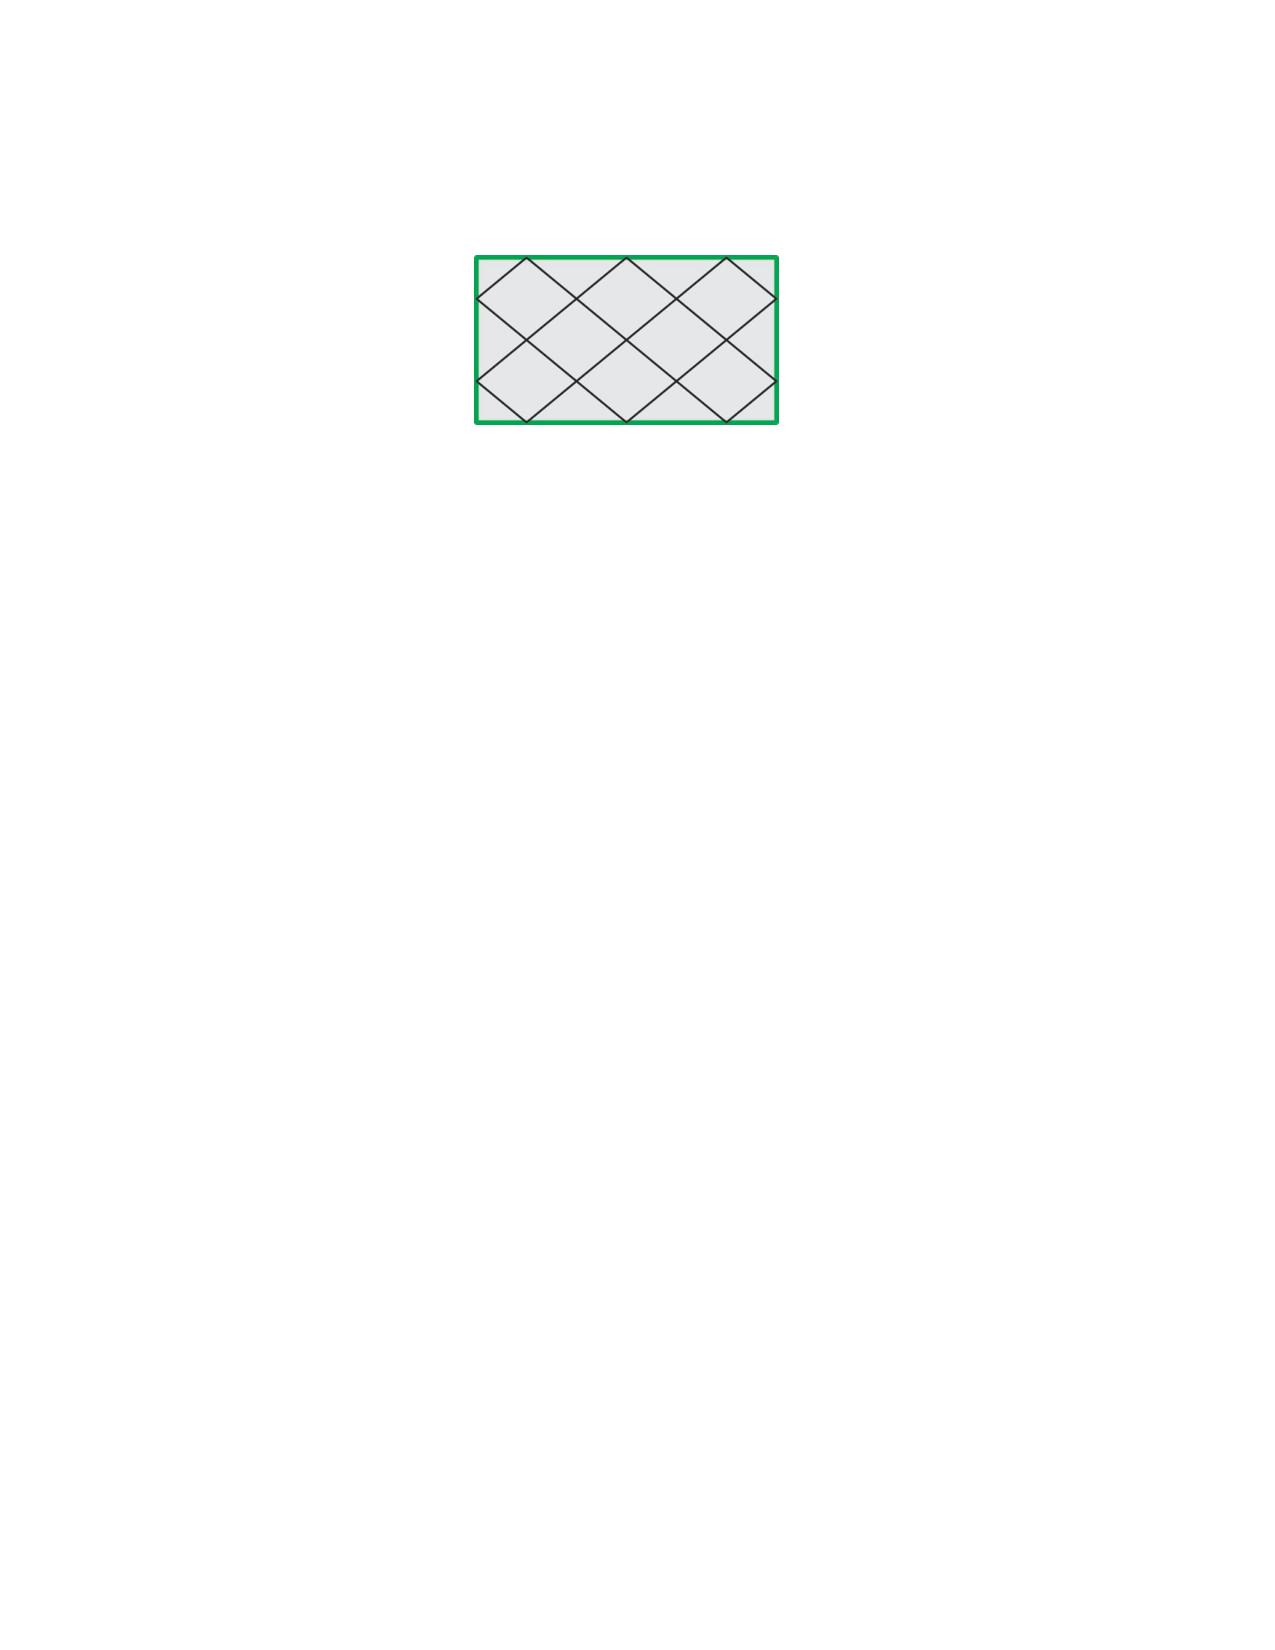
\includegraphics[width=1\linewidth]{1}
		\caption{\small\textit{\color{duongvaotoanhoc}Hình $1$. Quy ước về góc của nếp gấp trong origami hình học.}}
		\vspace*{-10pt}
	\end{figure}
	Với mỗi một hình origami, ở trạng thái bất kỳ, ta luôn có thể cắt xung quanh một đỉnh bằng một hình cầu. Khi trải phần bị cắt ra ta sẽ luôn được một hình tròn với các nếp gấp lồi và lõm (Hình $1$).
		\begin{figure}[H]
		\vspace*{-5pt}
		\centering
		\captionsetup{labelformat= empty, justification=centering}
		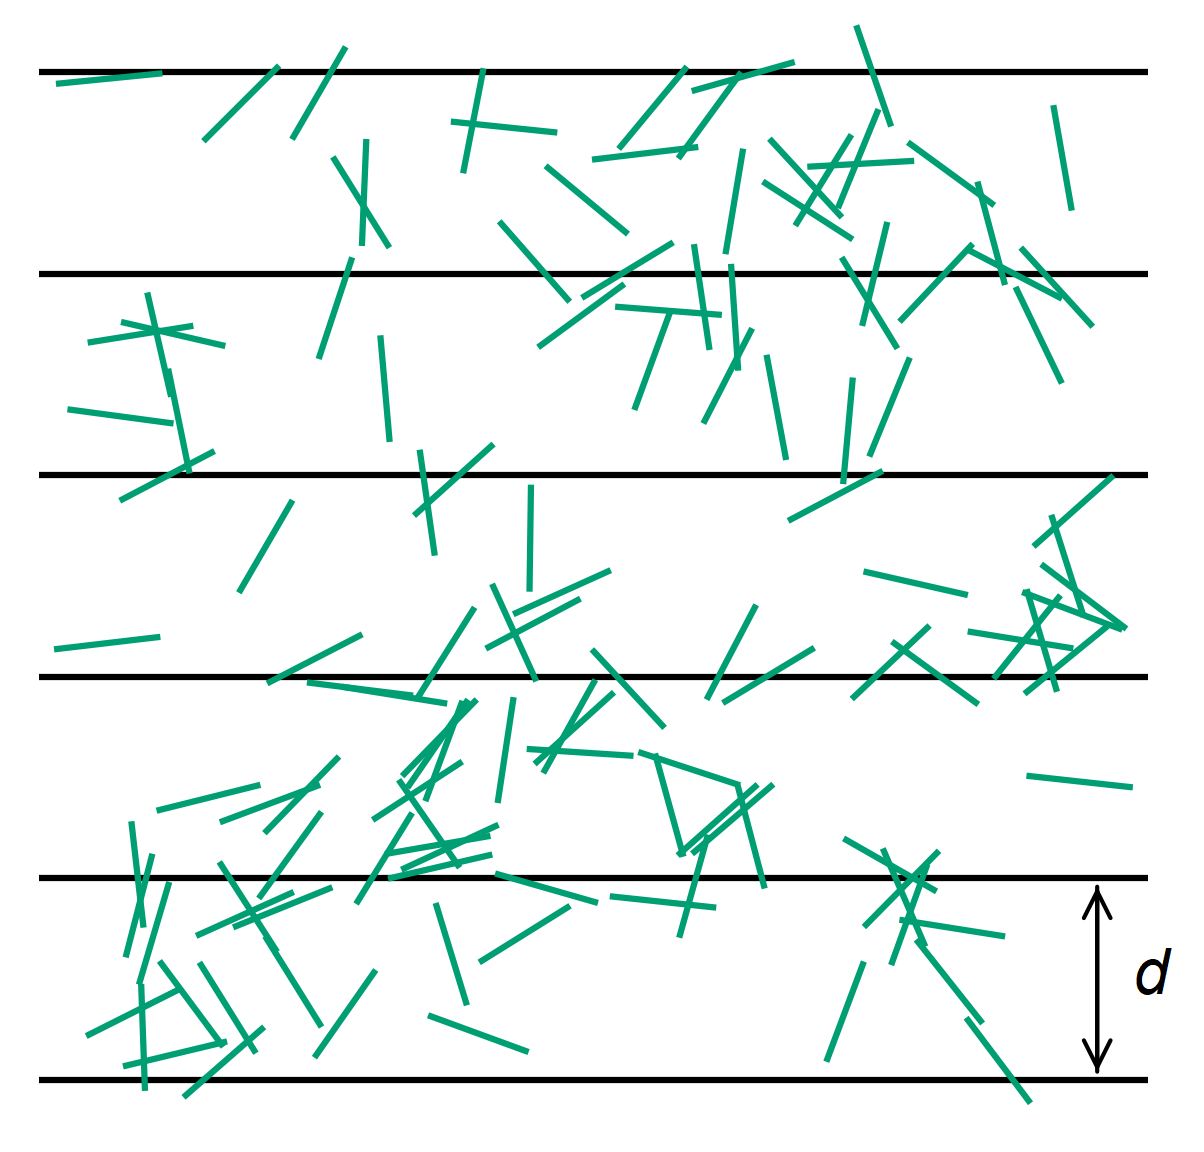
\includegraphics[width=1\linewidth]{2}
		\caption{\small\textit{\color{duongvaotoanhoc}Hình $2$. Cắt một đỉnh trong origami ra và trải ra, ta được hình tròn với các nếp gấp như hình bên phải. Chú ý: nét liền là nếp gấp lồi, nét đứt là nếp gấp lõm.}}
		\vspace*{-10pt}
	\end{figure}
		\begin{figure}[H]
		\vspace*{-5pt}
		\centering
		\captionsetup{labelformat= empty, justification=centering}
		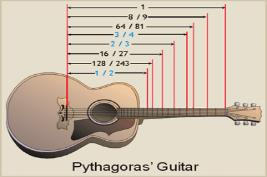
\includegraphics[width=1\linewidth]{3}
		\caption{\small\textit{\color{duongvaotoanhoc}Hình $3$. Các góc liên quan đến một đỉnh trong trường hợp đỉnh bậc $4$ (có $4$ nếp gấp kết nối với đỉnh). Như đã quy ước, đường nét liền (màu xanh) là nếp gấp lồi, nét đứt (màu đỏ) là nếp gấp lõm).}}
		\vspace*{-10pt}
	\end{figure}
	Với mỗi một đỉnh được tạo như vậy, ta gọi các góc giữa các nếp gấp (lồi và lõm) kề nhau là $\alpha_1, \alpha_2,\ldots,\alpha_n$. Đồng thời, ta còn xét các góc liên quan đến các nếp gấp, ký hiệu là $\gamma_1, \gamma_2,\ldots,\gamma_n$. Có thể dễ dàng nhận thấy, dù cho hình origami ở bất kỳ trạng thái nào, kể cả các trạng thái trung gian thì các cung tròn của hình tròn ban đầu đều nằm trên một \linebreak hình cầu, các góc $\alpha$ không đổi nhưng các góc $\gamma$ sẽ thay đổi trong quá trình gấp.
	\vskip 0.05cm
	Nếu xoay hướng nhìn mặt cầu, thì hình ở bên phải của Hình $3$ sẽ có dạng như trong Hình $4$. Ta kẻ thêm một dây cung trên mặt cầu (trong mặt phẳng đi qua tâm hình cầu) để chia góc $\gamma_3$ ra thành $\phi$ và $\psi$.
		\begin{figure}[H]
		\vspace*{-5pt}
		\centering
		\captionsetup{labelformat= empty, justification=centering}
		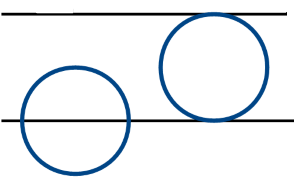
\includegraphics[width=1\linewidth]{4}
		\caption{\small\textit{\color{duongvaotoanhoc}Hình $4$. Mặt cầu khi nhìn từ phía ngoài vào. Các góc $\alpha$ sẽ ứng với các dây cung trên mặt cầu còn các góc $\gamma$ ứng với các điểm đại diện cho nếp gấp trên mặt cầu.}}
		\vspace*{-5pt}
	\end{figure}
	Sử dụng công thức định lý hàm số cosin cho tam giác cầu, ta có:
	\begin{align*}
		&\cos\zeta \\[-0.5ex]
		= \,&\cos \alpha_1\cos\alpha_2 + \sin\alpha_1\sin\alpha_2\cos(\pi - \gamma_2)
	\end{align*}
	và
	\begin{align*}
		&\cos\zeta \\[-0.5ex]
		= \,&\cos\alpha_3\cos\alpha_4 + \sin \alpha_3\sin\alpha_4 \cos(\pi - \gamma_4).
	\end{align*}
	Đồng thời, áp dụng điều kiện Kawasaki -- \linebreak Justin, ta có: $\alpha_3 = \pi - \alpha_1$ và $\alpha_4=\pi-\alpha_2$. Thay vào các công thức trên và trừ đi nhau ta được:
	\begin{align*}
		\sin\alpha_1\sin\alpha_2(\cos\gamma_2 - \cos\gamma_4) = 0.
	\end{align*}
	Do $\alpha_1$ và $\alpha_2$ đều khác $0$ nên ta có:
	\begin{align*}
		\cos \gamma_2 = \cos\gamma_4.
	\end{align*}
	Tương tự:
	\vskip 0.05cm
		\centerline{$\cos\gamma_1 = \cos\gamma_3$.}
	\vskip 0.05cm
		\textbf{\color{toanhocdoisong}Điều kiện Kawasaki--Justin:} Khi hình được trải phẳng được gấp lại hoàn toàn, nếu ta đi theo mép của đường tròn ban đầu, ta được một vòng kín, do đó, tổng của các góc mà ta đi theo một chiều (ngược hoặc xuôi kim đồng hồ) cũng bằng với tổng của các góc khi ta đi theo chiều ngược lại. Hiển nhiên $\theta_1 + \theta_2 + \ldots + \theta_n = 2\pi$ nên:
		\begin{align*}
			\sum\limits_{i \text{\,\,chẵn}} \theta_i  = \sum\limits_{i \text{\,\,lẻ}} \theta_i = \pi.
		\end{align*}
		\begin{figure}[H]
	\vspace*{-5pt}
	\centering
	\captionsetup{labelformat= empty, justification=centering}
	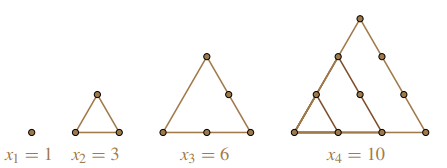
\includegraphics[width=0.9\linewidth]{5}
	\vspace*{-10pt}
\end{figure}
	Sau đó, ta cần tiến hành xét dấu tùy theo trường hợp lồi lõm của các nếp gấp. Như với Hình $3$ và Hình $4$, ta sẽ có:
	\begin{align*}
		\gamma_2 = \gamma_4 = \gamma_+.
	\end{align*}
	và
	\begin{align*}
		\gamma_1 = -\gamma_3 = \gamma_-.
	\end{align*}
	Cách làm trên cho ta quan hệ giữa các góc $\gamma$ đối nhau. Ta hãy tiếp tục tìm quan hệ giữa các góc $\gamma$ kề nhau trong trường hợp đỉnh bậc $4$. Ta có:
	\begin{align*}
		\sin \gamma_3 &= \sin \left(\pi - (\phi + \psi)\right) \\[-0.5ex]
		&= \sin\phi\cos\psi + \cos\phi \sin\psi.
	\end{align*}
	Theo định lý hàm số sin cho tam giác cầu:
	\begin{align*}
		\frac{\sin\phi}{\sin\alpha_1} = \frac{\sin\gamma_2}{\sin\zeta},\frac{\sin\psi}{\sin\alpha_4} = \frac{\sin \gamma_4}{\sin\zeta}.
	\end{align*}
	Theo định lý hàm số cosin cho tam giác cầu:
	\begin{align*}
		&\cos\alpha_1 = \cos\alpha_2\cos\zeta + \sin\alpha_2\sin\zeta\cos\phi,\\[-0.5ex] &\cos\alpha_4 = \cos\alpha_3\cos\zeta + \sin\alpha_3\sin\zeta\cos\psi.
	\end{align*}
	Dùng các định nghĩa $\gamma_+, \gamma_-$ như ở trên, ta có thể đơn giản hóa biểu thức của $\sin\gamma_3$ thành:
	\begin{align*}
		\sin\gamma_- = \frac{\cos\alpha_2 - \cos\alpha_1}{1 - \cos\zeta}\sin\gamma_+.
	\end{align*}
	Thay biểu thức: $\cos\zeta = \cos\alpha_1\cos\alpha_2 - \sin\alpha_1\sin\alpha_2\cos\gamma_+$,
	ta được:
	\begin{align*}
		&\sin\gamma_- \\[-0.5ex]
		= &\frac{\cos\alpha_2 \!-\! \cos\alpha_1}{1\!-\!\left(\!\cos\!\alpha_1\!\cos\!\alpha_2 \!-\! \sin\!\alpha_1\!\sin\!\alpha_2\!\cos\!\gamma_+\!\!\right)}\!\sin\gamma_+.
	\end{align*}
	Sử dụng phép thế Weierstrass (biểu diễn các giá trị lượng giác của $x$ theo $\tan\frac{x}{2}$), ta đặt:
	\begin{align*}
		t_+ = \tan\frac{\gamma_+}{2}, t_- = \frac{\gamma_-}{2}
	\end{align*}
	và rút gọn để được:
	\begin{align*}
		t_+ = t_- \frac{\sin\frac{1}{2}\left(\alpha_1 + \alpha_2\right)}{\sin\frac{1}{2}\left(\alpha_1 - \alpha_2\right)}
	\end{align*}
	hay:
	\begin{align*}
		\frac{\tan\frac{1}{2}\gamma_+}{\tan\frac{1}{2}\gamma_-} = \frac{\sin\frac{1}{2}\left(\alpha_1 + \alpha_2\right)}{\sin\frac{1}{2}\left(\alpha_1 - \alpha_2\right)} = \mu.
	\end{align*}
	Trong kết quả này, vế phải là một hằng số tại mỗi đỉnh trong quá trình gấp, gọi là bội số góc nếp gấp. Do đó, với lưới các đỉnh bậc $4$ như ta đang xét, ta chỉ cần một tham số duy nhất để biểu diễn trạng thái của toàn bộ cấu trúc. Thật vậy, nếu ta biết được một góc ứng với một nếp gấp bất kỳ, ta có thể tính được tất cả các góc của các nếp gấp cùng đỉnh cũng như tất cả các góc ứng với bất kỳ nếp gấp nào khác trong cấu trúc. Tuy nhiên, việc này lại yêu cầu cách gấp phải thỏa mãn một số điều kiện toán học nhất định.
	\vskip 0.05cm
	$\pmb{2.}$ \textbf{\color{toanhocdoisong}Khả năng gấp cứng}
	\vskip 0.05cm
	Như ta đã thấy với Miura--ori, khi ta kéo/đẩy cấu trúc ở hai góc thì các nếp gấp trong cấu trúc sẽ chuyển động theo tác động của ta đến bất kỳ trạng thái nào. Đây được gọi là khả năng gấp cứng (rigid foldability): cấu trúc có thể chuyển động liên tục giữa các trạng thái mà 
	\vskip 0.05cm
	-- vị trí các đỉnh so với tờ giấy không bị dịch chuyển; 
	\vskip 0.05cm
	-- các nếp gấp luôn là đường thẳng với độ dài không bị thay đổi;
	\vskip 0.05cm
	-- các mặt giấy (phần được xác định với biên là các nếp gấp) luôn phẳng, không bị uốn cong, không bị thay đổi về hình dạng và diện tích.
	\vskip 0.05cm
	Nói cách khác, việc chuyển trạng thái trong trường hợp này chỉ thay đổi các góc $\gamma$ trong cấu trúc.
	\vskip 0.05cm
	Vậy một cách gấp như thế nào sẽ có thể thỏa mãn những điều kiệu này?
	\vskip 0.05cm
	Ta hãy nhìn lại biểu thức của $\frac{\tan\frac{1}{2}\gamma_+}{\tan\frac{1}{2}\gamma_-}$. Với bất cứ thiết kế nào của đỉnh bậc $4$ mà $\gamma_2$ và $\gamma_4$ cùng dấu còn $\gamma_1$ và $\gamma_3$ ngược dấu, ta luôn có giá trị của biểu thức này $> 1$. Hàm số $\tan$ là hàm số đơn điệu cho nên với tất cả các trạng thái của nếp gấp:
	\begin{align*}
		&|\gamma_-| < |\gamma_+| \text{  với  } \gamma \in (0,\pi),\\
		&|\gamma_-| = |\gamma_+| \text{ với } \gamma = 0,\pi.
	\end{align*}
	Dấu bằng chỉ xảy ra ở trạng thái các mặt giấy đồng phẳng hoặc đè hoàn toàn lên nhau. Do quan hệ trên mà các nếp gấp ứng với $\gamma_+$ được gọi là các nếp gấp chính còn các nếp gấp ứng với $\gamma_-$ được gọi là các nếp gấp phụ (độ lớn của góc tương ứng bé hơn).
	\vskip 0.05cm
	Với mỗi đỉnh, ta có thể biểu diễn mối quan hệ giữa các nếp gấp gắn với đỉnh đó bằng một đồ thị có hướng. Mỗi nếp gấp được coi là một đỉnh của đồ thị (chú ý: phân biệt với đỉnh của cấu trúc origami). Giữa hai nếp gấp kề nhau, ta tạo một cạnh của đồ thị, cạnh này có hướng từ nếp gấp chính đến nếp gấp phụ (Hình $5$).
		\begin{figure}[H]
		\vspace*{-5pt}
		\centering
		\captionsetup{labelformat= empty, justification=centering}
		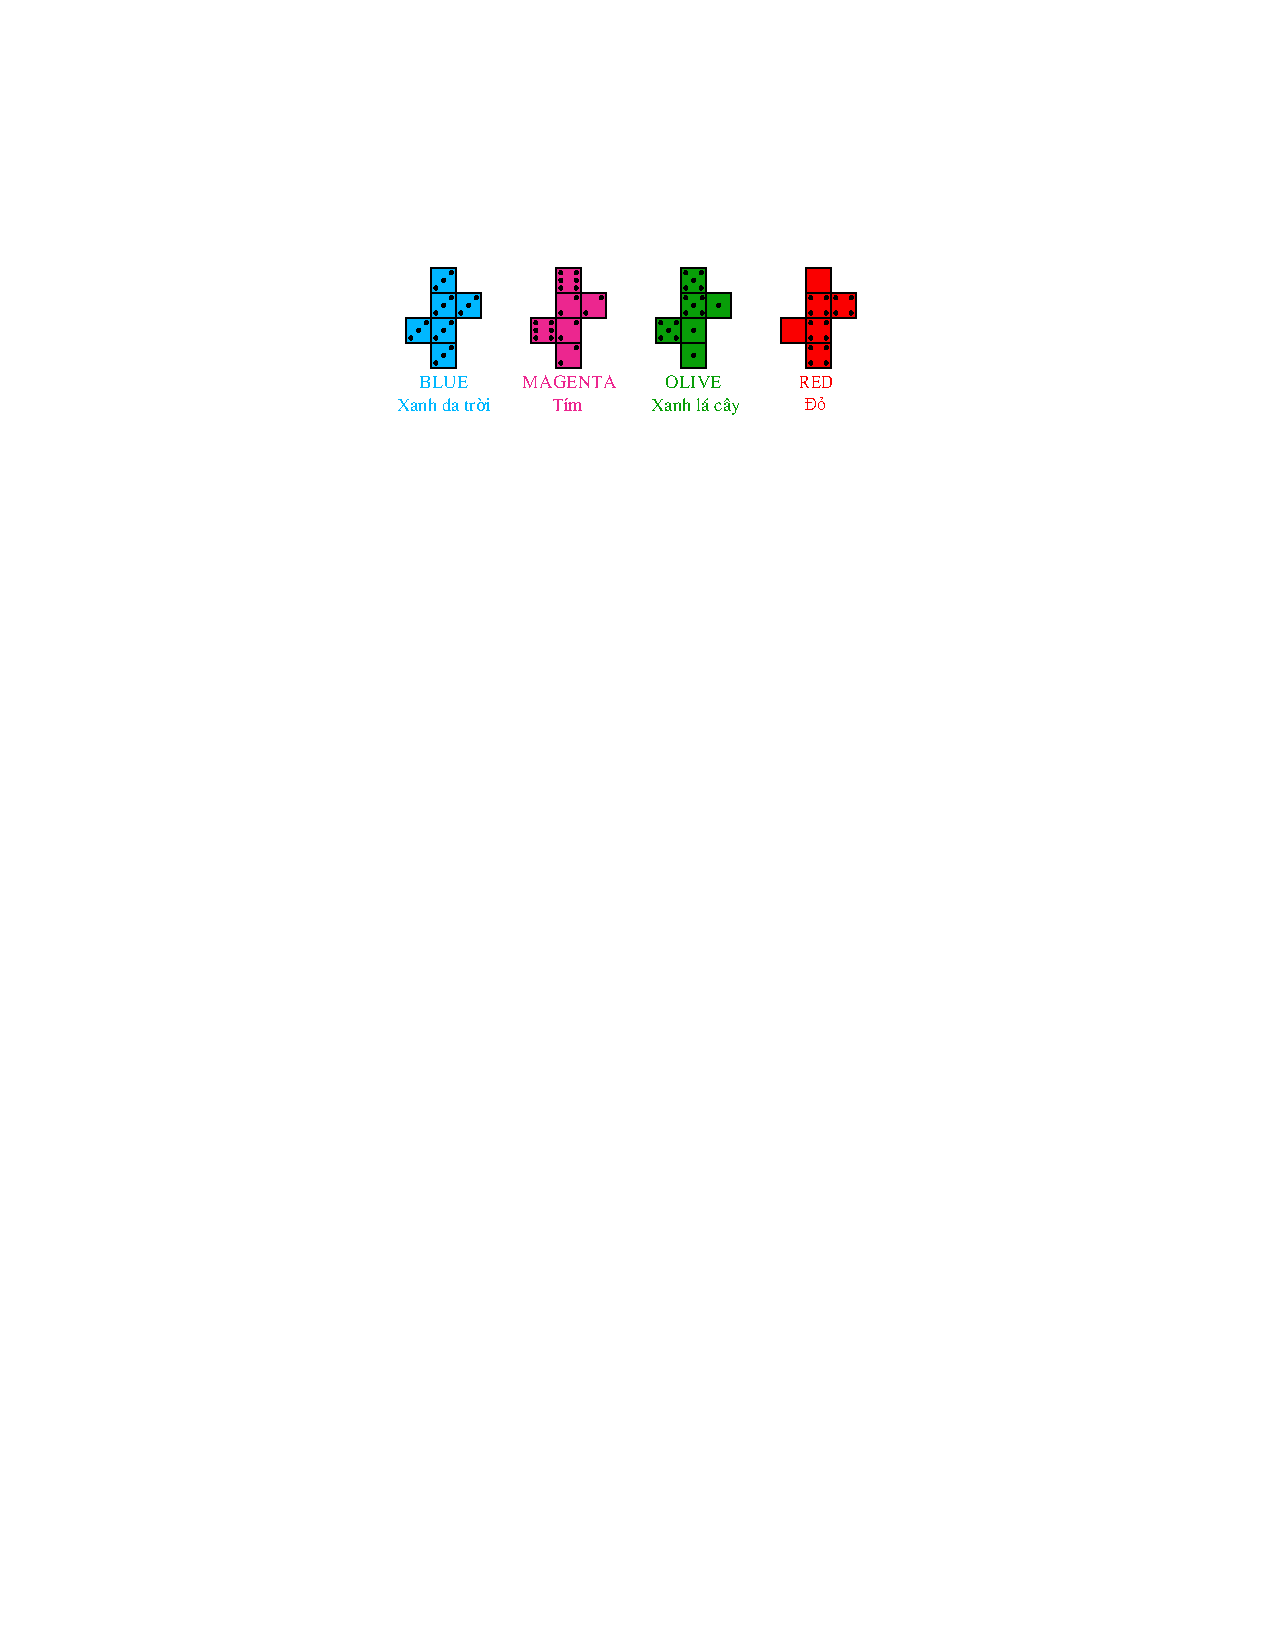
\includegraphics[width=0.8\linewidth]{6}
		\caption{\small\textit{\color{duongvaotoanhoc}Hình $5$. Đồ thị có hướng của một đỉnh. Cạnh của đồ thị nối các nếp gấp kề nhau và đi từ một nếp gấp chính đến một nếp gấp phụ.}}
		\vspace*{-10pt}
	\end{figure}
	Tất nhiên cấu trúc origami của ta không chỉ có một đỉnh. Các đỉnh được nối với nhau bằng các nếp gấp. Do đó, với mỗi nếp gấp \linebreak(đỉnh của đồ thị có hướng), ta vẽ được hai \linebreak cạnh đến hai nếp gấp khác. Đồ thị đã bao gồm tất cả các cạnh từ các nếp gấp được gọi là đồ thị góc nếp gấp của cấu trúc origami. Đồ thị này sẽ thay đổi với những cách gấp khác nhau. Hình $6$ biểu diễn các cách gấp khác nhau của $4$ đỉnh có bậc $4$ cùng đồ thị có hướng được dựng từ chúng. Ở đây, ta ký hiệu nếp gấp lồi là $M$, nếp gấp lõm là $V$ (theo tiếng Anh, $M$ -- mountain, $V$ -- valley). Các cách gấp từ trái sang sẽ được ký hiệu là $M^4$, $M^2 V^2$, và $(MV)^2$ theo dạng lồi lõm của các cạnh nối $4$ đỉnh đang xét.
	\vskip 0.05cm
	Đồ thị có hướng mà ta đã lập sẽ cho biết quan hệ về độ lớn giữa các góc của các nếp gấp trong cấu trúc origami. Với cách gấp $M^4$, từ đồ thị ta có:
	\begin{align*}
		\gamma_a > \gamma_b > \gamma_c > \gamma_d > \gamma_a
	\end{align*}
	Điều này là không thể vì góc ứng với nếp gấp $a$ không thể lớn hơn chính nó. Do đó nếp gấp này không thể có trạng thái trung gian giữa trạng thái phẳng và trạng thái gập dẹt. Nếu ta thử gấp, một số mặt giấy sẽ bị cong hoặc biến dạng.
	\begin{figure}[H]
		\vspace*{-5pt}
		\centering
		\captionsetup{labelformat= empty, justification=centering}
		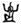
\includegraphics[width=1\linewidth]{7}
		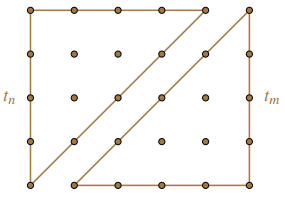
\includegraphics[width=1\linewidth]{8}
		\caption{\small\textit{\color{duongvaotoanhoc}Hình $6$. Trên: các cách gấp $M^4$, $M^2 V^2$, và $(MV)^2$ với $4$ đỉnh bậc $4$. Dưới: đồ thị có hướng của chúng. Các nếp gấp nối các đỉnh trong $4$ đỉnh được xét được ký hiệu là $\gamma_a, \gamma_b, \gamma_c$ và $\gamma_d$.}}
		\vspace*{-5pt}
	\end{figure}
	Với cách gấp $(MV)^2$, ta cũng gặp trường hợp không khả thi như vậy:
	\begin{align*}
		\gamma_a<\gamma_b<\gamma_c<\gamma_d<\gamma_a.
	\end{align*}
	Trong khi đó, dạng $M^2 V^2$ (ở giữa) có quan hệ từ đồ thị luôn luôn được thỏa mãn:
	\begin{align*}
		\gamma_a,\gamma_c>\gamma_b,\gamma_d.
	\end{align*} 
	Các quan hệ từ đồ thị này giúp ta nhận diện những cách gấp không có khả năng gấp cứng. Tuy nhiên, nó không phải là điều kiện đủ. Ở phần trước, ta đã thiết lập được bội số $\mu$ biểu diễn quan hệ giữa các góc của các nếp gấp. Bội số này có thể được bổ sung làm trọng số cho các cạnh của đồ thị có hướng của ta sau khi bổ sung thêm dấu phụ thuộc vào dấu của các góc $\gamma$ (Hình $7$). Khi các hàm số tan ứng với hai góc $\frac{1}{2}\gamma$ trái dấu thì trọng số sẽ âm.
	\vskip 0.05cm
	Ví dụ cho trường hợp $M^4$, từ đồ thị ta có (chú ý chiều của cạnh đồ thị khi viết biểu thức):
	\begin{align*}
		&\mu_a = \frac{\tan\frac{1}{2}\gamma_a}{\tan\frac{1}{2}\gamma_d},\mu_b = \frac{\tan\frac{1}{2}\gamma_b}{\tan\frac{1}{2}\gamma_a},\\
		& \mu_c= \frac{\tan\frac{1}{2}\gamma_c}{\tan\frac{1}{2}\gamma_b}, \mu_d = \frac{\tan\frac{1}{2}\gamma_d}{\tan\frac{1}{2}\gamma_a}.
	\end{align*}
	Do đó:
	\begin{align*}
		\mu_a\mu_b\mu_c\mu_d = 1.
	\end{align*}
	Do các giá trị $\mu$ luôn lớn hơn $1$, biểu thức này luôn không thỏa mãn.
	\begin{figure}[H]
		\vspace*{-5pt}
		\centering
		\captionsetup{labelformat= empty, justification=centering}
		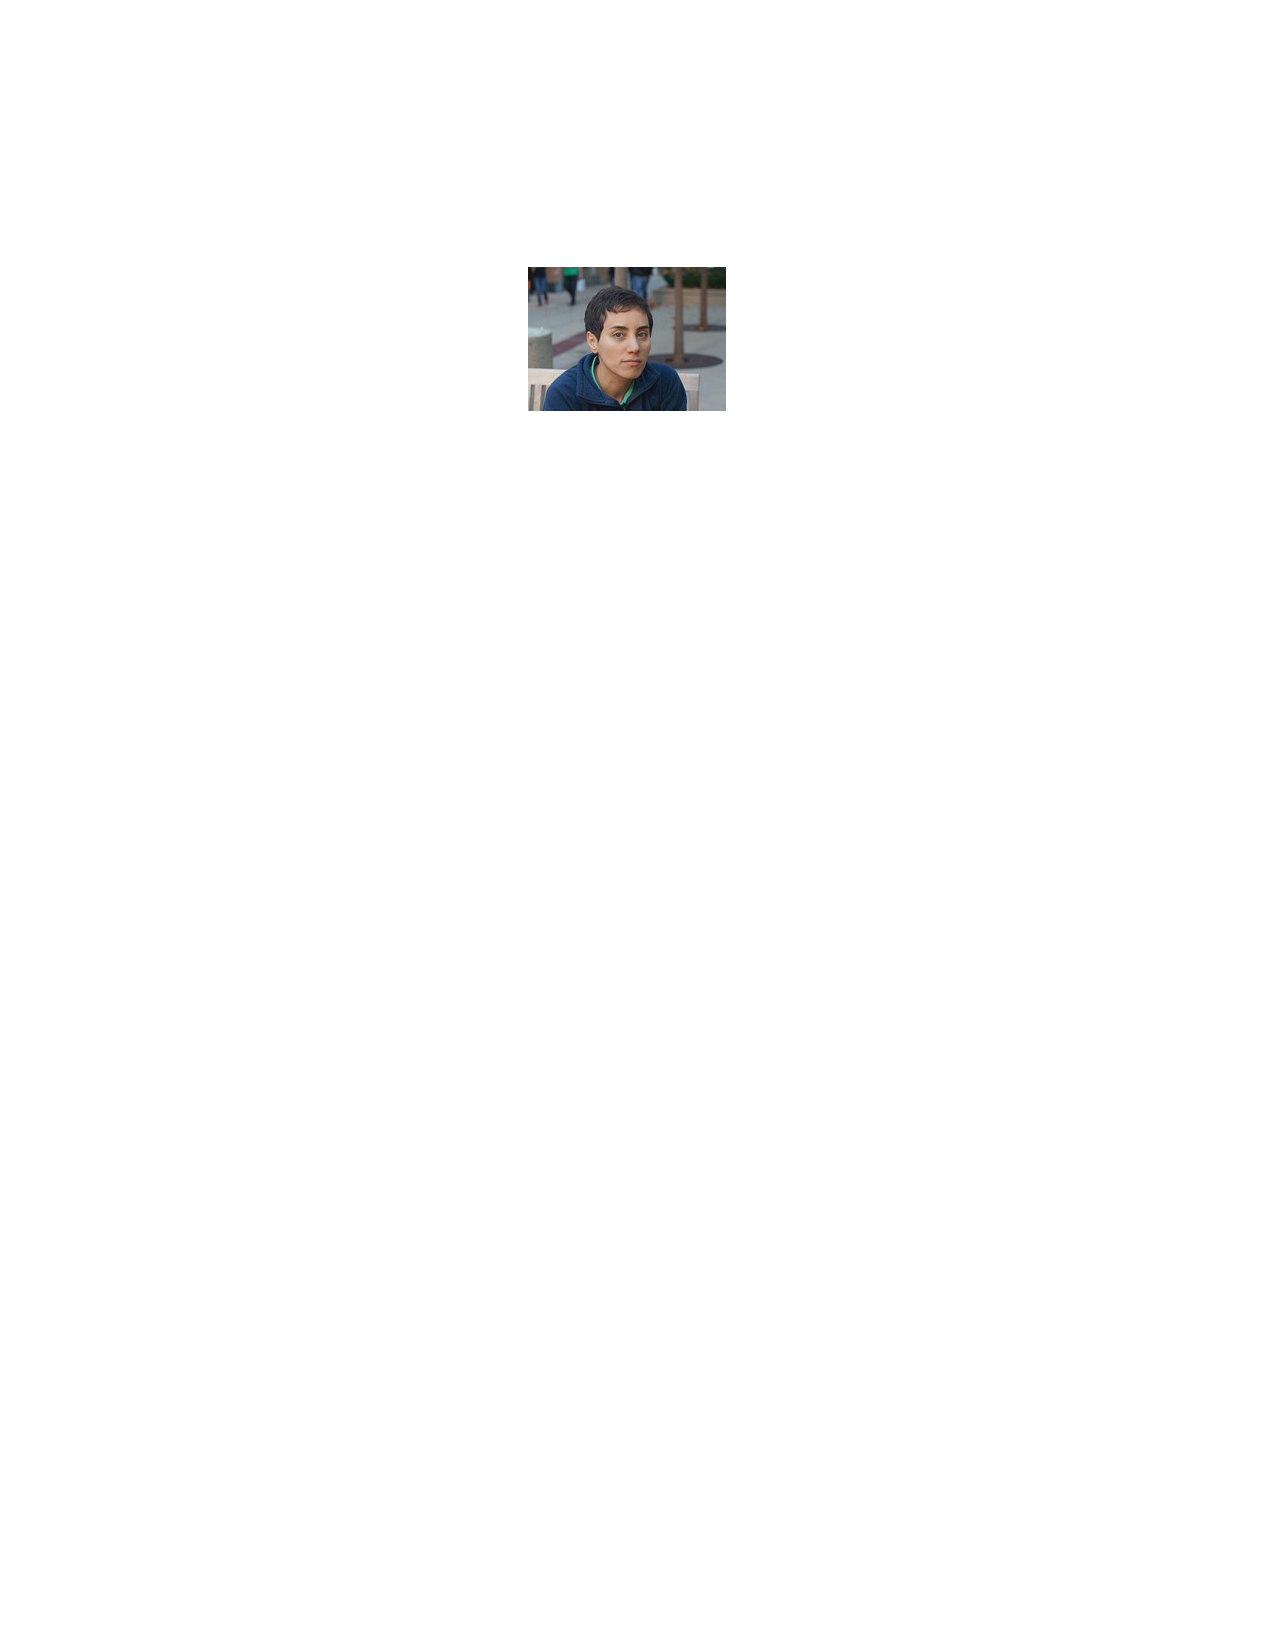
\includegraphics[width=1\linewidth]{9}
		\caption{\quad$M^4$				\hspace*{75pt}		$(MV)^2$}
		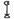
\includegraphics[width=1\linewidth]{10}
		\caption{$M^2 V^2$ \hspace*{65pt}					$M^3 V$}
		\caption{\small\textit{\color{duongvaotoanhoc}	Hình $7$. Đồ thị có trọng số cho các cách gấp. (Các góc $\gamma$ không ghi ở đây nhưng giống với hình $6$).}}
		\vspace*{-10pt}
	\end{figure}
	Nếu quy ước chiều dương là chiều ngược kim đồng hồ, ta có thể viết biểu thức cho các vòng khuyên trong đồ thị nhanh hơn thay vì liệt kê các quan hệ như trên. Với cạnh cùng chiều với chiều dương, ta giữ nguyên trọng số còn cạnh ngược chiều dương ta lấy nghịch đảo của trọng số. Với trường hợp $(MV)^2$, ta có:
	\begin{align*}
		\left(-\mu_a^{-1}\right)\left(-\mu_b^{-1}\right)\left(-\mu_c^{-1}\right)\left(-\mu_d^{-1}\right) = 1.
	\end{align*}
	Quan hệ này cũng không thể thỏa mãn do các giá trị $\mu$ luôn lớn hơn $1$.
	\vskip 0.05cm
	Với trường hợp $M^2 V^2$ (Miura--ori là một dạng này), ta có:
	\begin{align*}
		\left(-\mu_a^{-1}\right)\mu_b\left(-\mu_c^{-1}\right)\mu_d = 1.
	\end{align*}
	Với cấu trúc mà các đỉnh được gấp với các góc ở đỉnh giống nhau, các giá trị $\mu$ luôn bằng nhau và quan hệ trên luôn đúng. Đến đây ta có thể khẳng định dạng $M^2 V^2$ có thể gấp cứng.
	\vskip 0.05cm
	Tương tự với dạng $M^3 V$, ta có:
	\begin{align*}
		\left(-\mu_a^{-1}\right)\mu_b\mu_c \left(-\mu_d^{-1}\right)=1
	\end{align*}
	cũng luôn đúng và dạng này cũng có thể gấp cứng.
	\vskip 0.05cm
	Có thể thấy, việc sử dụng đồ thị để biểu diễn quan hệ giữa các nếp gấp giúp ta phân tích quan hệ giữa chúng một cách thuận tiện và có vai trò quan trọng trong việc tìm hiểu các  tính chất của cấu trúc origami.
	\vskip 0.05cm
	$\pmb{3.}$ \textbf{\color{toanhocdoisong}Bài toán đếm số cách gấp}
	\vskip 0.05cm
	Trong origami hình học, việc đếm và liệt kê số cách gấp (cách phân bố nếp gấp lồi/lõm từ một mẫu cho trước ví dụ như Miura--ori) là một bài toán khó. Dạng toán này xuất hiện trong nhiều nghiên cứu thực tiễn, ví dụ về các màng polymer. Tuy vậy, ngay cả bài toán tưởng như đơn giản như số cách gấp con tem bưu chính theo lưới chữ nhật cũng chưa có lời giải toán học chính xác (trong khi mỗi nếp gấp có thể là lồi hoặc lõm chứ không đồng bộ theo cả hàng hay cả cột).
	\vskip 0.05cm
	Mặc dù chưa có một lý thuyết tổng quát cho việc liệt kê các cách gấp có thể, với một số họ nếp gấp, bài toán này có thể giải quyết được. Chúng ta hãy xét trường hợp cho Miura--ori. Miura--ori có $6$ cách phân bố nếp gấp lồi/lõm (Hình $8$). 
		\begin{figure}[H]
		\vspace*{5pt}
		\centering
		\captionsetup{labelformat= empty, justification=centering}
		\includegraphics[height=0.32\linewidth]{11a}
		\includegraphics[height=0.32\linewidth]{11b}
		\caption{\small\textit{\color{duongvaotoanhoc}Hình $8$. Bên trái: $6$ cách phân bố lồi lõm của Miura--ori. Nét đậm là nếp gấp lồi, nét nhạt là nếp gấp lõm. Bên phải: Gấp tờ giấy làm $4$ với Miura--ori. }}
		\vspace*{-10pt}
	\end{figure}
	Tại sao lại chỉ có $6$? Đó là bởi theo định lý Maekawa--Justin, số nếp gấp lồi và lõm ở một đỉnh bao giờ cũng lệch nhau $2$ đơn vị ($M-V=±2$). Thật vậy, ở trạng thái các nếp gấp đã được gập dẹt lại (ngược với trường hợp trải phẳng), các góc $\gamma$ sẽ nhận giá trị $\pi$ hoặc $-\pi$ tùy theo nếp gấp là lồi hoặc lõm. Vì các dây cung tạo thành một vòng kín, tổng của các góc $\gamma$ phải bằng một số nguyên lần của $2\pi$ và do đó ta có chênh lệch $2$ nếp gấp.
	\vskip 0.05cm
	Với trường hợp đơn giản nhất, nếu ta gấp tờ giấy thành $4$ với Miura--ori, ta sẽ chỉ có một đỉnh và tờ giấy được chia thành $2$ hàng và $2$ cột. Số cách gấp sẽ là $6$.
	\vskip 0.05cm 
	Xét trường hợp tờ giấy được gấp thành $2$ hàng và $n$ cột. Như ở trên, $M(2,2)=6$. Giả sử đã chọn được cách sắp xếp cho $(n-1)$ cột ban đầu, thì cột thứ $n$ chỉ còn $3$ cách chọn (do nếp gấp lồi chỉ nối được với nếp gấp lồi của đỉnh bên cạnh, tương tự cho nếp gấp lõm). Do đó ta có: 
	\begin{align*}
		M(2,n)=3M(2,n-1).
	\end{align*}
	Từ công thức truy hồi này ta được: $M(2,n)=2\cdot3^{n-1}$.
	\vskip 0.05cm
	Với các trường hợp phức tạp hơn, lập luận có phần hơi dài và rắc rối nên không được trình bày ở đây. Bạn đọc quan tâm đến dạng chứng minh tổ hợp này có thể tham khảo (Hull, $2003$) và (Ginepro \& Hull, $2014$).
	\vskip 0.05cm
	Với trường hợp $m$ hàng và $3$ cột, kết quả như sau:
	\begin{align*}
		M(m,3) = c_+ \left(\frac{1}{\alpha_+}\right)^m + c_-\left(\frac{1}{\alpha_-}\right)^m
	\end{align*}
	với $\alpha_{\pm} = \frac{5 \pm \sqrt{17}}{4}$ và $c_{\pm} = \frac{17 \pm 3\sqrt{17}}{34}$.
	\vskip 0.05cm
 	Kết quả cho một số trường hợp $m$ hàng và $n$ cột như sau:
	\begin{table}[H]
		\setlength{\tabcolsep}{3pt}
		\renewcommand{\arraystretch}{1.2}
		\resizebox{\columnwidth}{!}{\begin{tabular}{|c|c|c|c|c|}
			\hline
			$m/n$ & $2$ & $3$ & $4$ & $5$\\
			\hline
			$2$ & $6$ & $18$ & $54$ & $162$\\
			\hline
			$3$ & $18$ & $82$ & $374$ & $1706$\\
			\hline
			$4$ & $54$ & $374$ & $2604$ & $18150$\\
			\hline
			$5$ & $162$ & $1706$ & $18150$ & $193662$\\
			\hline
			$6$ & $486$ & $7782$ & $126534$ & $2068146$\\
			\hline
			$7$ & $1458$& $35498$ & $882180$& $22091514$\\
			\hline
			$8$ & $4374$ & $161926$ & $6150510$ & $235994086$\\
			\hline
		\end{tabular}}
	\end{table}
	Một điều đáng chú ý là các kết quả này giống với số cách dùng $3$ màu để tô lưới chữ nhật ($m$ hàng và $n$ cột) sao cho không có hai ô liền nhau (dọc hoặc ngang) có cùng màu và ô đầu tiên đã được tô. Với việc các nếp gấp từ các đỉnh liền nhau phải khớp với nhau, điều này cũng không quá ngạc nhiên. Bạn đọc có thể xem chi tiết chứng minh tương đương giữa hai bài toán này trong (Ginepro \& Hull, $2014$).
	\vskip 0.05cm
	$\pmb{4.}$ \textbf{\color{toanhocdoisong}Origami hình học và các công nghệ tương lai}
	\vskip 0.05cm
	Dù chỉ mới được phát triển trong vài thập kỷ qua, origami hình học đã cho thấy khả năng liên kết mạnh mẽ với nhiều ngành khoa học khác nhau. Không chỉ giúp tạo nên những vật liệu gọn hơn, bền chắc hơn như đã thấy trong các phần trước, các lý thuyết này còn đóng vai trò quan trọng trong các nghiên cứu liên ngành khác nhau trong các lĩnh vực mũi nhọn của công nghệ.
	\vskip 0.1cm
	Những robot thiết kế nhờ origami hình học có thể thay đổi hình dạng tùy theo hoàn \linebreak cảnh có nhiều tiềm năng về ứng dụng, đặc biệt trong lĩnh vực cứu hộ. Chúng cũng có thể được kết hợp với trí tuệ nhân tạo, cho ra các cỗ máy vừa thông minh vừa linh hoạt.
	\vskip 0.05cm
	Ứng dụng origami hình học vào công nghệ nano cũng giúp chế tạo các vật liệu có thể thay đổi hình dạng với kích thước rất nhỏ và hình dạng thay đổi phụ thuộc vào điều kiện môi trường (xung điện kích hoạt, nhiệt độ, độ ẩm, ...). Những vật liệu như vậy có nhiều ứng dụng trong cuộc sống  ví dụ như giúp cho thuốc được giải phóng trong cơ thể người ở vị trí chính xác hơn hay trong tương lai không xa là những robot công nghệ nano có khả năng tự gấp lại.
	\begin{figure}[H]
		\vspace*{-5pt}
		\centering
		\captionsetup{labelformat= empty, justification=centering}
		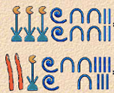
\includegraphics[width=1\linewidth]{13}
		\caption{\small\textit{\color{duongvaotoanhoc}Hình $9$. Robot thiết kế nhờ origami hình học với hình dạng thay đổi.}}
		\vspace*{-10pt}
	\end{figure}
	Có thể nói, sự phát triển mạnh mẽ của \linebreak origami hình học cho thấy vai trò của toán học ứng dụng trong nghệ thuật, công nghệ lẫn đời sống con người.
	\vskip 0.05cm
	\textbf{\color{toanhocdoisong}Tài liệu tham khảo}
	\vskip 0.05cm
	[$1$] Felton, S., Tolley, M., Demaine, E., Rus, D., \& Wood, R. ($2014$, Aug). Applied origami. A method for building self--folding machines. \textit{Science}, $644-6$.
	\vskip 0.05cm
	[$2$] Ginepro, J., \& Hull, T. C. ($2014$). Counting Miura--ori Foldings. \textit{Journal of Integer Sequences}, $17$.
	\vskip 0.05cm
	[$3$] Hull, T. ($2003$). Counting Mountain--Valley Assignments for Flat Folds. \textit{Ars Combinatoria}, $67$, $175-188$.
	\vskip 0.05cm
	[$4$] Lang, R. J. ($2009$). \textit{Origami$4$}. AK Peters.
	\vskip 0.05cm
	[$5$] Lang, R. J. ($2018$). \textit{Twists, Tilings, and Tessellations. Mathematical Methods for Geometric Origami}. CRC Press.
	\vskip 0.05cm
	[$6$] Tachi, T., \& Hull, T. C. ($2017$, April). Self--Foldability of Rigid Origami. \textit{Journal of Mechanisms and Robotics}, $9$.
\end{multicols}
